%Erzeugt mit dem LaTeX-Generator: http://latex.sehnot.de

%Schriftgr��e, Layout, Papierformat, Art des Dokumentes
\documentclass[11pt,oneside,a4paper, bibtotoc]{scrartcl}

%Einstellungen der Seitenr�nder
\usepackage[left=3cm,right=4cm,top=3cm,bottom=3cm,includeheadfoot]{geometry}
 
%neue Rechtschreibung
\usepackage[ngerman]{babel}
 
%Umlaute erm�glichen
\usepackage[latin1]{inputenc}
  
%Grafiken einbinden 
\usepackage{graphicx}
 
%Das Abbildungsverzeichnis in das Inhaltsverzeichnis einbinden
\usepackage[nottoc]{tocbibind}

\usepackage[printonlyused]{acronym}  

%Verlinkungen
\usepackage{hyperref} 

%Absatzeinr�cken vermeiden}
\parindent 0pt

%Kopf- und Fu�zeile  
\usepackage{fancyhdr}  
\pagestyle{fancy}   
\fancyhf{}
   
%Kopfzeile links bzw. innen
\fancyhead[L]{\nouppercase{\leftmark}}
%Linie oben
\renewcommand{\headrulewidth}{0.5pt}
 
%Fu�zeile rechts bzw. au�en
\fancyfoot[R]{\thepage}
%Linie unten
\renewcommand{\footrulewidth}{0.5pt}
 

%Deckblatt
\begin{document}
%Nummeriungstiefe Kapitel
\setcounter{secnumdepth}{4}

%Nummerierungstiefe Inhaltsverzeichnis
\setcounter{tocdepth}{4}
\begin{titlepage} 
\author{Oliver Stannarius \\ und \\Roman M�ller} 
\title{Projekt \\ Service Oriented Computing} 
\date{\today}  
\maketitle
\thispagestyle{empty}
\end{titlepage}

%Inhaltsverzeichnis
\tableofcontents
\pagenumbering{Roman}
\newpage
\pagenumbering{arabic}

%Einleitung
\section{Einleitung}
\setcounter{page}{1}
jetzt gehts los
%Beispiel f�r ein Bild einf�gen
%\begin{figure}[htbp]
 % \centering
	%\ac{KDE}
  %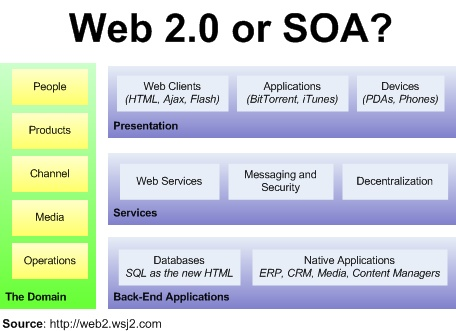
\includegraphics{web2soa.jpg}  
    
  %\caption[Titel f�r das Verzeichnis]{Titel}
  %\label{Labelname}
%\end{figure}
\newpage

%Grundlagen 
\section{Grundlagen}

\subsection{Service Orientierung}
\subsubsection{Definition}
Eine genaue Definition f�r SOA gibt es nicht. Die ersten die den Begriff
verwendeten war die Gartner Group, welche den Begriff wie folgt definieren:
\\

Service-oriented architecture (SOA) is a client/server software design approach
in which an application consists of software services and software service
consumers (also known as clients or service requesters). SOA differs from the
more general client/server model in its definitive emphasis on loose coupling
between software components, and in its use of separately standing interfaces.\\
SOA principles are rendered during application design, development and
deployment. These renditions share the essential principles of encapsulation
and flexible coupling, but they differ in detail. The fundamental intent of
SOA is the non-intrusive reuse of software components (services) in new
runtime contexts. The design and development of SOA is performed for the
purpose of achieving such an agile runtime environment. \cite{Natis:2003}  

\subsubsection{Grundlegende Konzepte}
\subsubsection{Aufbau}  
 
\subsection{WebService}  
\subsubsection{Definition}
\subsubsection{WebService Architektur} 
\subsubsection{WebService Standards}
\paragraph{WSDL}
\paragraph{SOAP}
\paragraph{UDDI}
 
\subsection{BPEL4WS}
\subsubsection{Definition}
\subsubsection{Variablen und XPath}
\subsubsection{Sprachbestandteile}
\paragraph{Basic Activities}
\paragraph{Structured Activities} 
\paragraph{Scopes}

 
 
\newpage

%Teilaufgabe 1
\section{Existierende reale Web Services}
\subsection{webservice 1 (name)}
\subsubsection{Beschreibung}
\subsubsection{Nutzung des WebService (name)}
\subsection{webservice 2 (name)}
\subsubsection{Beschreibung}
\subsubsection{Nutzung des WebService (name)}
 
\newpage 

%Teilaufgabe 2
\section{Entwicklung von 2 \glqq realistischen\grqq \ BPEL Prozesse}
\newpage

%Teilaufgabe 3
\section{BPRules}
\newpage

%Zusammenfassung
\section{Zusammenfassung}






%Abk�rzungsverzeichnis
\newpage      
\section{Abk�rzungsverzeichnis} 
\begin{acronym}[LINUX]

 \acro{KDE}{K Desktop Environment} 
 \acro{SQL}{Structured Query Language} 
 \acro{Bash}{Bourne-again shell}
\end{acronym} 

%Quellenverzeichnis 
\newpage 
 
\bibliographystyle{alphadin}  
\bibliography{quellen}  %name der .bib Datei 

%Abbildungsverzeichnis
\newpage
\listoffigures 
 
\end{document}
